% Created by tikzDevice version 0.12.6 on 2025-08-19 18:35:36
% !TEX encoding = UTF-8 Unicode
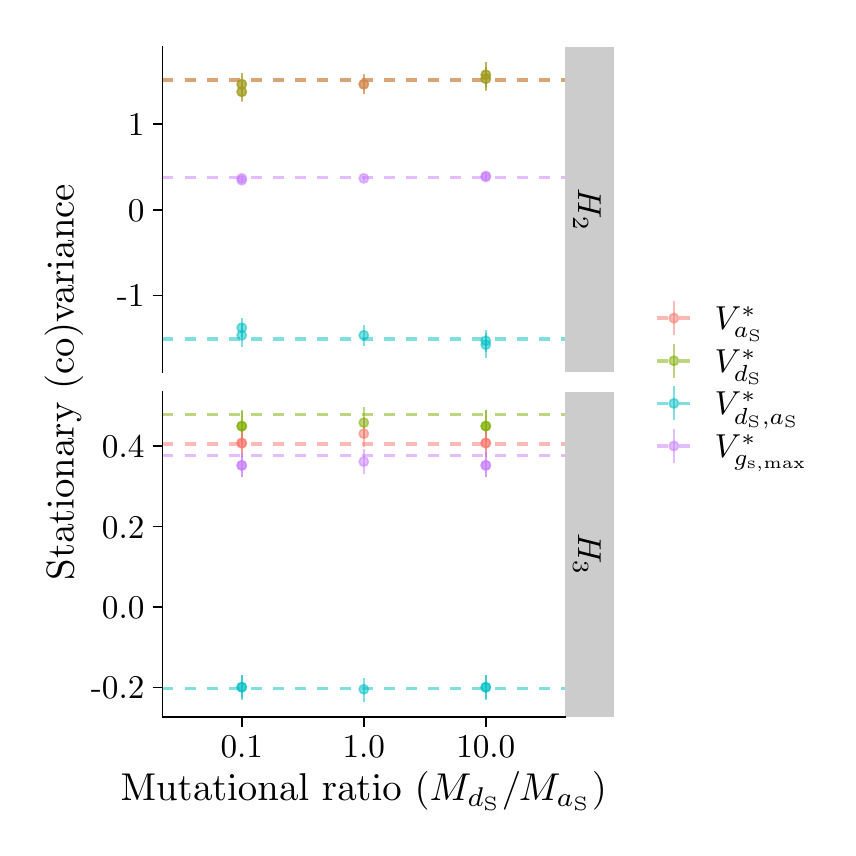
\begin{tikzpicture}[x=1pt,y=1pt]
\definecolor{fillColor}{RGB}{255,255,255}
\path[use as bounding box,fill=fillColor,fill opacity=0.00] (0,0) rectangle (289.08,289.08);
\begin{scope}
\path[clip] ( 48.69,164.52) rectangle (194.20,282.08);
\definecolor{drawColor}{RGB}{124,174,0}

\path[draw=drawColor,draw opacity=0.50,line width= 1.3pt,dash pattern=on 4pt off 4pt ,line join=round] ( 48.69,270.08) -- (194.20,270.08);
\definecolor{drawColor}{RGB}{248,118,109}

\path[draw=drawColor,draw opacity=0.50,line width= 1.3pt,dash pattern=on 4pt off 4pt ,line join=round] ( 48.69,270.08) -- (194.20,270.08);
\definecolor{drawColor}{RGB}{0,191,196}

\path[draw=drawColor,draw opacity=0.50,line width= 1.3pt,dash pattern=on 4pt off 4pt ,line join=round] ( 48.69,176.49) -- (194.20,176.49);
\definecolor{drawColor}{RGB}{199,124,255}

\path[draw=drawColor,draw opacity=0.50,line width= 1.3pt,dash pattern=on 4pt off 4pt ,line join=round] ( 48.69,234.98) -- (194.20,234.98);
\definecolor{drawColor}{RGB}{248,118,109}

\path[draw=drawColor,draw opacity=0.50,line width= 0.7pt,line join=round] (165.54,267.51) -- (165.54,276.74);
\definecolor{drawColor}{RGB}{124,174,0}

\path[draw=drawColor,draw opacity=0.50,line width= 0.7pt,line join=round] (165.54,267.63) -- (165.54,276.60);
\definecolor{drawColor}{RGB}{0,191,196}

\path[draw=drawColor,draw opacity=0.50,line width= 0.7pt,line join=round] (165.54,169.86) -- (165.54,178.74);
\definecolor{drawColor}{RGB}{248,118,109}

\path[draw=drawColor,draw opacity=0.50,line width= 0.7pt,line join=round] (165.54,266.39) -- (165.54,274.89);
\definecolor{drawColor}{RGB}{124,174,0}

\path[draw=drawColor,draw opacity=0.50,line width= 0.7pt,line join=round] (165.54,266.37) -- (165.54,274.72);
\definecolor{drawColor}{RGB}{0,191,196}

\path[draw=drawColor,draw opacity=0.50,line width= 0.7pt,line join=round] ( 77.35,173.76) -- ( 77.35,181.84);

\path[draw=drawColor,draw opacity=0.50,line width= 0.7pt,line join=round] (165.54,171.96) -- (165.54,179.99);
\definecolor{drawColor}{RGB}{248,118,109}

\path[draw=drawColor,draw opacity=0.50,line width= 0.7pt,line join=round] ( 77.35,264.67) -- ( 77.35,272.66);
\definecolor{drawColor}{RGB}{124,174,0}

\path[draw=drawColor,draw opacity=0.50,line width= 0.7pt,line join=round] ( 77.35,264.93) -- ( 77.35,272.84);
\definecolor{drawColor}{RGB}{0,191,196}

\path[draw=drawColor,draw opacity=0.50,line width= 0.7pt,line join=round] (121.45,174.03) -- (121.45,181.49);
\definecolor{drawColor}{RGB}{248,118,109}

\path[draw=drawColor,draw opacity=0.50,line width= 0.7pt,line join=round] ( 77.35,262.14) -- ( 77.35,269.46);
\definecolor{drawColor}{RGB}{124,174,0}

\path[draw=drawColor,draw opacity=0.50,line width= 0.7pt,line join=round] (121.45,265.02) -- (121.45,272.24);
\definecolor{drawColor}{RGB}{248,118,109}

\path[draw=drawColor,draw opacity=0.50,line width= 0.7pt,line join=round] (121.45,265.17) -- (121.45,272.15);
\definecolor{drawColor}{RGB}{124,174,0}

\path[draw=drawColor,draw opacity=0.50,line width= 0.7pt,line join=round] ( 77.35,262.52) -- ( 77.35,269.37);
\definecolor{drawColor}{RGB}{0,191,196}

\path[draw=drawColor,draw opacity=0.50,line width= 0.7pt,line join=round] ( 77.35,177.41) -- ( 77.35,184.21);
\definecolor{drawColor}{RGB}{199,124,255}

\path[draw=drawColor,draw opacity=0.50,line width= 0.7pt,line join=round] (165.54,234.40) -- (165.54,236.69);

\path[draw=drawColor,draw opacity=0.50,line width= 0.7pt,line join=round] (165.54,234.16) -- (165.54,236.22);

\path[draw=drawColor,draw opacity=0.50,line width= 0.7pt,line join=round] ( 77.35,233.63) -- ( 77.35,235.65);

\path[draw=drawColor,draw opacity=0.50,line width= 0.7pt,line join=round] (121.45,233.72) -- (121.45,235.59);

\path[draw=drawColor,draw opacity=0.50,line width= 0.7pt,line join=round] ( 77.35,233.07) -- ( 77.35,234.76);
\definecolor{drawColor}{RGB}{248,118,109}
\definecolor{fillColor}{RGB}{248,118,109}

\path[draw=drawColor,draw opacity=0.50,line width= 0.6pt,line join=round,line cap=round,fill=fillColor,fill opacity=0.50] (165.54,272.04) circle (  1.69);
\definecolor{drawColor}{RGB}{124,174,0}
\definecolor{fillColor}{RGB}{124,174,0}

\path[draw=drawColor,draw opacity=0.50,line width= 0.6pt,line join=round,line cap=round,fill=fillColor,fill opacity=0.50] (165.54,272.05) circle (  1.69);
\definecolor{drawColor}{RGB}{0,191,196}
\definecolor{fillColor}{RGB}{0,191,196}

\path[draw=drawColor,draw opacity=0.50,line width= 0.6pt,line join=round,line cap=round,fill=fillColor,fill opacity=0.50] (165.54,174.53) circle (  1.69);
\definecolor{drawColor}{RGB}{248,118,109}
\definecolor{fillColor}{RGB}{248,118,109}

\path[draw=drawColor,draw opacity=0.50,line width= 0.6pt,line join=round,line cap=round,fill=fillColor,fill opacity=0.50] (165.54,270.62) circle (  1.69);
\definecolor{drawColor}{RGB}{124,174,0}
\definecolor{fillColor}{RGB}{124,174,0}

\path[draw=drawColor,draw opacity=0.50,line width= 0.6pt,line join=round,line cap=round,fill=fillColor,fill opacity=0.50] (165.54,270.66) circle (  1.69);
\definecolor{drawColor}{RGB}{0,191,196}
\definecolor{fillColor}{RGB}{0,191,196}

\path[draw=drawColor,draw opacity=0.50,line width= 0.6pt,line join=round,line cap=round,fill=fillColor,fill opacity=0.50] ( 77.35,177.93) circle (  1.69);

\path[draw=drawColor,draw opacity=0.50,line width= 0.6pt,line join=round,line cap=round,fill=fillColor,fill opacity=0.50] (165.54,175.93) circle (  1.69);
\definecolor{drawColor}{RGB}{248,118,109}
\definecolor{fillColor}{RGB}{248,118,109}

\path[draw=drawColor,draw opacity=0.50,line width= 0.6pt,line join=round,line cap=round,fill=fillColor,fill opacity=0.50] ( 77.35,268.65) circle (  1.69);
\definecolor{drawColor}{RGB}{124,174,0}
\definecolor{fillColor}{RGB}{124,174,0}

\path[draw=drawColor,draw opacity=0.50,line width= 0.6pt,line join=round,line cap=round,fill=fillColor,fill opacity=0.50] ( 77.35,268.64) circle (  1.69);
\definecolor{drawColor}{RGB}{0,191,196}
\definecolor{fillColor}{RGB}{0,191,196}

\path[draw=drawColor,draw opacity=0.50,line width= 0.6pt,line join=round,line cap=round,fill=fillColor,fill opacity=0.50] (121.45,177.92) circle (  1.69);
\definecolor{drawColor}{RGB}{248,118,109}
\definecolor{fillColor}{RGB}{248,118,109}

\path[draw=drawColor,draw opacity=0.50,line width= 0.6pt,line join=round,line cap=round,fill=fillColor,fill opacity=0.50] ( 77.35,265.93) circle (  1.69);
\definecolor{drawColor}{RGB}{124,174,0}
\definecolor{fillColor}{RGB}{124,174,0}

\path[draw=drawColor,draw opacity=0.50,line width= 0.6pt,line join=round,line cap=round,fill=fillColor,fill opacity=0.50] (121.45,268.64) circle (  1.69);
\definecolor{drawColor}{RGB}{248,118,109}
\definecolor{fillColor}{RGB}{248,118,109}

\path[draw=drawColor,draw opacity=0.50,line width= 0.6pt,line join=round,line cap=round,fill=fillColor,fill opacity=0.50] (121.45,268.66) circle (  1.69);
\definecolor{drawColor}{RGB}{124,174,0}
\definecolor{fillColor}{RGB}{124,174,0}

\path[draw=drawColor,draw opacity=0.50,line width= 0.6pt,line join=round,line cap=round,fill=fillColor,fill opacity=0.50] ( 77.35,265.92) circle (  1.69);
\definecolor{drawColor}{RGB}{0,191,196}
\definecolor{fillColor}{RGB}{0,191,196}

\path[draw=drawColor,draw opacity=0.50,line width= 0.6pt,line join=round,line cap=round,fill=fillColor,fill opacity=0.50] ( 77.35,180.65) circle (  1.69);
\definecolor{drawColor}{RGB}{199,124,255}
\definecolor{fillColor}{RGB}{199,124,255}

\path[draw=drawColor,draw opacity=0.50,line width= 0.6pt,line join=round,line cap=round,fill=fillColor,fill opacity=0.50] (165.54,235.48) circle (  1.69);

\path[draw=drawColor,draw opacity=0.50,line width= 0.6pt,line join=round,line cap=round,fill=fillColor,fill opacity=0.50] (165.54,235.14) circle (  1.69);

\path[draw=drawColor,draw opacity=0.50,line width= 0.6pt,line join=round,line cap=round,fill=fillColor,fill opacity=0.50] ( 77.35,234.62) circle (  1.69);

\path[draw=drawColor,draw opacity=0.50,line width= 0.6pt,line join=round,line cap=round,fill=fillColor,fill opacity=0.50] (121.45,234.62) circle (  1.69);

\path[draw=drawColor,draw opacity=0.50,line width= 0.6pt,line join=round,line cap=round,fill=fillColor,fill opacity=0.50] ( 77.35,233.95) circle (  1.69);
\end{scope}
\begin{scope}
\path[clip] ( 48.69, 39.96) rectangle (194.20,157.52);
\definecolor{drawColor}{RGB}{124,174,0}

\path[draw=drawColor,draw opacity=0.50,line width= 1.3pt,dash pattern=on 4pt off 4pt ,line join=round] ( 48.69,149.24) -- (194.20,149.24);
\definecolor{drawColor}{RGB}{248,118,109}

\path[draw=drawColor,draw opacity=0.50,line width= 1.3pt,dash pattern=on 4pt off 4pt ,line join=round] ( 48.69,138.54) -- (194.20,138.54);
\definecolor{drawColor}{RGB}{0,191,196}

\path[draw=drawColor,draw opacity=0.50,line width= 1.3pt,dash pattern=on 4pt off 4pt ,line join=round] ( 48.69, 50.35) -- (194.20, 50.35);
\definecolor{drawColor}{RGB}{199,124,255}

\path[draw=drawColor,draw opacity=0.50,line width= 1.3pt,dash pattern=on 4pt off 4pt ,line join=round] ( 48.69,134.54) -- (194.20,134.54);
\definecolor{drawColor}{RGB}{124,174,0}

\path[draw=drawColor,draw opacity=0.50,line width= 0.7pt,line join=round] (165.54,139.22) -- (165.54,150.96);

\path[draw=drawColor,draw opacity=0.50,line width= 0.7pt,line join=round] ( 77.35,139.24) -- ( 77.35,150.95);

\path[draw=drawColor,draw opacity=0.50,line width= 0.7pt,line join=round] ( 77.35,139.09) -- ( 77.35,150.69);

\path[draw=drawColor,draw opacity=0.50,line width= 0.7pt,line join=round] (121.45,140.92) -- (121.45,152.18);

\path[draw=drawColor,draw opacity=0.50,line width= 0.7pt,line join=round] (165.54,139.90) -- (165.54,150.99);
\definecolor{drawColor}{RGB}{248,118,109}

\path[draw=drawColor,draw opacity=0.50,line width= 0.7pt,line join=round] ( 77.35,134.07) -- ( 77.35,144.35);

\path[draw=drawColor,draw opacity=0.50,line width= 0.7pt,line join=round] (121.45,137.38) -- (121.45,147.62);

\path[draw=drawColor,draw opacity=0.50,line width= 0.7pt,line join=round] ( 77.35,133.79) -- ( 77.35,143.93);

\path[draw=drawColor,draw opacity=0.50,line width= 0.7pt,line join=round] (165.54,133.81) -- (165.54,143.89);

\path[draw=drawColor,draw opacity=0.50,line width= 0.7pt,line join=round] (165.54,133.98) -- (165.54,143.75);
\definecolor{drawColor}{RGB}{199,124,255}

\path[draw=drawColor,draw opacity=0.50,line width= 0.7pt,line join=round] (121.45,127.64) -- (121.45,136.85);
\definecolor{drawColor}{RGB}{0,191,196}

\path[draw=drawColor,draw opacity=0.50,line width= 0.7pt,line join=round] (165.54, 46.11) -- (165.54, 55.03);
\definecolor{drawColor}{RGB}{199,124,255}

\path[draw=drawColor,draw opacity=0.50,line width= 0.7pt,line join=round] (165.54,126.77) -- (165.54,135.68);
\definecolor{drawColor}{RGB}{0,191,196}

\path[draw=drawColor,draw opacity=0.50,line width= 0.7pt,line join=round] ( 77.35, 46.22) -- ( 77.35, 55.08);

\path[draw=drawColor,draw opacity=0.50,line width= 0.7pt,line join=round] (121.45, 45.30) -- (121.45, 54.09);
\definecolor{drawColor}{RGB}{199,124,255}

\path[draw=drawColor,draw opacity=0.50,line width= 0.7pt,line join=round] ( 77.35,126.72) -- ( 77.35,135.43);
\definecolor{drawColor}{RGB}{0,191,196}

\path[draw=drawColor,draw opacity=0.50,line width= 0.7pt,line join=round] (165.54, 46.44) -- (165.54, 55.03);
\definecolor{drawColor}{RGB}{199,124,255}

\path[draw=drawColor,draw opacity=0.50,line width= 0.7pt,line join=round] ( 77.35,126.59) -- ( 77.35,135.14);
\definecolor{drawColor}{RGB}{0,191,196}

\path[draw=drawColor,draw opacity=0.50,line width= 0.7pt,line join=round] ( 77.35, 46.77) -- ( 77.35, 55.28);
\definecolor{drawColor}{RGB}{199,124,255}

\path[draw=drawColor,draw opacity=0.50,line width= 0.7pt,line join=round] (165.54,126.81) -- (165.54,135.32);
\definecolor{drawColor}{RGB}{124,174,0}
\definecolor{fillColor}{RGB}{124,174,0}

\path[draw=drawColor,draw opacity=0.50,line width= 0.6pt,line join=round,line cap=round,fill=fillColor,fill opacity=0.50] (165.54,145.13) circle (  1.69);

\path[draw=drawColor,draw opacity=0.50,line width= 0.6pt,line join=round,line cap=round,fill=fillColor,fill opacity=0.50] ( 77.35,145.12) circle (  1.69);

\path[draw=drawColor,draw opacity=0.50,line width= 0.6pt,line join=round,line cap=round,fill=fillColor,fill opacity=0.50] ( 77.35,145.03) circle (  1.69);

\path[draw=drawColor,draw opacity=0.50,line width= 0.6pt,line join=round,line cap=round,fill=fillColor,fill opacity=0.50] (121.45,146.36) circle (  1.69);

\path[draw=drawColor,draw opacity=0.50,line width= 0.6pt,line join=round,line cap=round,fill=fillColor,fill opacity=0.50] (165.54,145.11) circle (  1.69);
\definecolor{drawColor}{RGB}{248,118,109}
\definecolor{fillColor}{RGB}{248,118,109}

\path[draw=drawColor,draw opacity=0.50,line width= 0.6pt,line join=round,line cap=round,fill=fillColor,fill opacity=0.50] ( 77.35,138.97) circle (  1.69);

\path[draw=drawColor,draw opacity=0.50,line width= 0.6pt,line join=round,line cap=round,fill=fillColor,fill opacity=0.50] (121.45,142.36) circle (  1.69);

\path[draw=drawColor,draw opacity=0.50,line width= 0.6pt,line join=round,line cap=round,fill=fillColor,fill opacity=0.50] ( 77.35,138.97) circle (  1.69);

\path[draw=drawColor,draw opacity=0.50,line width= 0.6pt,line join=round,line cap=round,fill=fillColor,fill opacity=0.50] (165.54,139.00) circle (  1.69);

\path[draw=drawColor,draw opacity=0.50,line width= 0.6pt,line join=round,line cap=round,fill=fillColor,fill opacity=0.50] (165.54,139.00) circle (  1.69);
\definecolor{drawColor}{RGB}{199,124,255}
\definecolor{fillColor}{RGB}{199,124,255}

\path[draw=drawColor,draw opacity=0.50,line width= 0.6pt,line join=round,line cap=round,fill=fillColor,fill opacity=0.50] (121.45,132.27) circle (  1.69);
\definecolor{drawColor}{RGB}{0,191,196}
\definecolor{fillColor}{RGB}{0,191,196}

\path[draw=drawColor,draw opacity=0.50,line width= 0.6pt,line join=round,line cap=round,fill=fillColor,fill opacity=0.50] (165.54, 50.73) circle (  1.69);
\definecolor{drawColor}{RGB}{199,124,255}
\definecolor{fillColor}{RGB}{199,124,255}

\path[draw=drawColor,draw opacity=0.50,line width= 0.6pt,line join=round,line cap=round,fill=fillColor,fill opacity=0.50] (165.54,130.93) circle (  1.69);
\definecolor{drawColor}{RGB}{0,191,196}
\definecolor{fillColor}{RGB}{0,191,196}

\path[draw=drawColor,draw opacity=0.50,line width= 0.6pt,line join=round,line cap=round,fill=fillColor,fill opacity=0.50] ( 77.35, 50.74) circle (  1.69);

\path[draw=drawColor,draw opacity=0.50,line width= 0.6pt,line join=round,line cap=round,fill=fillColor,fill opacity=0.50] (121.45, 50.01) circle (  1.69);
\definecolor{drawColor}{RGB}{199,124,255}
\definecolor{fillColor}{RGB}{199,124,255}

\path[draw=drawColor,draw opacity=0.50,line width= 0.6pt,line join=round,line cap=round,fill=fillColor,fill opacity=0.50] ( 77.35,130.93) circle (  1.69);
\definecolor{drawColor}{RGB}{0,191,196}
\definecolor{fillColor}{RGB}{0,191,196}

\path[draw=drawColor,draw opacity=0.50,line width= 0.6pt,line join=round,line cap=round,fill=fillColor,fill opacity=0.50] (165.54, 50.75) circle (  1.69);
\definecolor{drawColor}{RGB}{199,124,255}
\definecolor{fillColor}{RGB}{199,124,255}

\path[draw=drawColor,draw opacity=0.50,line width= 0.6pt,line join=round,line cap=round,fill=fillColor,fill opacity=0.50] ( 77.35,130.88) circle (  1.69);
\definecolor{drawColor}{RGB}{0,191,196}
\definecolor{fillColor}{RGB}{0,191,196}

\path[draw=drawColor,draw opacity=0.50,line width= 0.6pt,line join=round,line cap=round,fill=fillColor,fill opacity=0.50] ( 77.35, 50.79) circle (  1.69);
\definecolor{drawColor}{RGB}{199,124,255}
\definecolor{fillColor}{RGB}{199,124,255}

\path[draw=drawColor,draw opacity=0.50,line width= 0.6pt,line join=round,line cap=round,fill=fillColor,fill opacity=0.50] (165.54,130.93) circle (  1.69);
\end{scope}
\begin{scope}
\path[clip] (194.20,164.52) rectangle (211.80,282.08);
\definecolor{fillColor}{gray}{0.80}

\path[fill=fillColor] (194.20,164.52) rectangle (211.80,282.08);
\definecolor{drawColor}{RGB}{0,0,0}

\node[text=drawColor,rotate=-90.00,anchor=base,inner sep=0pt, outer sep=0pt, scale=  1.20] at (198.87,223.30) {$H_2$};
\end{scope}
\begin{scope}
\path[clip] (194.20, 39.96) rectangle (211.80,157.52);
\definecolor{fillColor}{gray}{0.80}

\path[fill=fillColor] (194.20, 39.96) rectangle (211.80,157.52);
\definecolor{drawColor}{RGB}{0,0,0}

\node[text=drawColor,rotate=-90.00,anchor=base,inner sep=0pt, outer sep=0pt, scale=  1.20] at (198.87, 98.74) {$H_3$};
\end{scope}
\begin{scope}
\path[clip] (  0.00,  0.00) rectangle (289.08,289.08);
\definecolor{drawColor}{RGB}{0,0,0}

\path[draw=drawColor,line width= 0.6pt,line join=round,line cap=rect] ( 48.69, 39.96) --
	(194.20, 39.96);
\end{scope}
\begin{scope}
\path[clip] (  0.00,  0.00) rectangle (289.08,289.08);
\definecolor{drawColor}{RGB}{0,0,0}

\path[draw=drawColor,line width= 0.6pt,line join=round] ( 77.35, 36.46) --
	( 77.35, 39.96);

\path[draw=drawColor,line width= 0.6pt,line join=round] (121.45, 36.46) --
	(121.45, 39.96);

\path[draw=drawColor,line width= 0.6pt,line join=round] (165.54, 36.46) --
	(165.54, 39.96);
\end{scope}
\begin{scope}
\path[clip] (  0.00,  0.00) rectangle (289.08,289.08);
\definecolor{drawColor}{RGB}{0,0,0}

\node[text=drawColor,anchor=base,inner sep=0pt, outer sep=0pt, scale=  1.20] at ( 77.35, 25.20) {0.1};

\node[text=drawColor,anchor=base,inner sep=0pt, outer sep=0pt, scale=  1.20] at (121.45, 25.20) {1.0};

\node[text=drawColor,anchor=base,inner sep=0pt, outer sep=0pt, scale=  1.20] at (165.54, 25.20) {10.0};
\end{scope}
\begin{scope}
\path[clip] (  0.00,  0.00) rectangle (289.08,289.08);
\definecolor{drawColor}{RGB}{0,0,0}

\path[draw=drawColor,line width= 0.6pt,line join=round,line cap=rect] ( 48.69,164.52) --
	( 48.69,282.08);
\end{scope}
\begin{scope}
\path[clip] (  0.00,  0.00) rectangle (289.08,289.08);
\definecolor{drawColor}{RGB}{0,0,0}

\node[text=drawColor,anchor=base east,inner sep=0pt, outer sep=0pt, scale=  1.20] at ( 42.19,188.15) {-1};

\node[text=drawColor,anchor=base east,inner sep=0pt, outer sep=0pt, scale=  1.20] at ( 42.19,219.15) {0};

\node[text=drawColor,anchor=base east,inner sep=0pt, outer sep=0pt, scale=  1.20] at ( 42.19,250.16) {1};
\end{scope}
\begin{scope}
\path[clip] (  0.00,  0.00) rectangle (289.08,289.08);
\definecolor{drawColor}{RGB}{0,0,0}

\path[draw=drawColor,line width= 0.6pt,line join=round] ( 45.19,192.28) --
	( 48.69,192.28);

\path[draw=drawColor,line width= 0.6pt,line join=round] ( 45.19,223.29) --
	( 48.69,223.29);

\path[draw=drawColor,line width= 0.6pt,line join=round] ( 45.19,254.29) --
	( 48.69,254.29);
\end{scope}
\begin{scope}
\path[clip] (  0.00,  0.00) rectangle (289.08,289.08);
\definecolor{drawColor}{RGB}{0,0,0}

\path[draw=drawColor,line width= 0.6pt,line join=round,line cap=rect] ( 48.69, 39.96) --
	( 48.69,157.52);
\end{scope}
\begin{scope}
\path[clip] (  0.00,  0.00) rectangle (289.08,289.08);
\definecolor{drawColor}{RGB}{0,0,0}

\node[text=drawColor,anchor=base east,inner sep=0pt, outer sep=0pt, scale=  1.20] at ( 42.19, 46.57) {-0.2};

\node[text=drawColor,anchor=base east,inner sep=0pt, outer sep=0pt, scale=  1.20] at ( 42.19, 75.61) {0.0};

\node[text=drawColor,anchor=base east,inner sep=0pt, outer sep=0pt, scale=  1.20] at ( 42.19,104.66) {0.2};

\node[text=drawColor,anchor=base east,inner sep=0pt, outer sep=0pt, scale=  1.20] at ( 42.19,133.71) {0.4};
\end{scope}
\begin{scope}
\path[clip] (  0.00,  0.00) rectangle (289.08,289.08);
\definecolor{drawColor}{RGB}{0,0,0}

\path[draw=drawColor,line width= 0.6pt,line join=round] ( 45.19, 50.70) --
	( 48.69, 50.70);

\path[draw=drawColor,line width= 0.6pt,line join=round] ( 45.19, 79.75) --
	( 48.69, 79.75);

\path[draw=drawColor,line width= 0.6pt,line join=round] ( 45.19,108.79) --
	( 48.69,108.79);

\path[draw=drawColor,line width= 0.6pt,line join=round] ( 45.19,137.84) --
	( 48.69,137.84);
\end{scope}
\begin{scope}
\path[clip] (  0.00,  0.00) rectangle (289.08,289.08);
\definecolor{drawColor}{RGB}{0,0,0}

\node[text=drawColor,anchor=base,inner sep=0pt, outer sep=0pt, scale=  1.40] at (121.45,  9.72) {Mutational ratio ($M_{d_\mathrm{S}} / M_{a_\mathrm{S}}$)};
\end{scope}
\begin{scope}
\path[clip] (  0.00,  0.00) rectangle (289.08,289.08);
\definecolor{drawColor}{RGB}{0,0,0}

\node[text=drawColor,rotate= 90.00,anchor=base,inner sep=0pt, outer sep=0pt, scale=  1.40] at ( 16.64,161.02) {Stationary (co)variance};
\end{scope}
\begin{scope}
\path[clip] (  0.00,  0.00) rectangle (289.08,289.08);
\definecolor{drawColor}{RGB}{248,118,109}

\path[draw=drawColor,draw opacity=0.50,line width= 1.3pt,dash pattern=on 4pt off 4pt ,line join=round] (227.34,184.12) -- (239.66,184.12);
\end{scope}
\begin{scope}
\path[clip] (  0.00,  0.00) rectangle (289.08,289.08);
\definecolor{drawColor}{RGB}{248,118,109}

\path[draw=drawColor,draw opacity=0.50,line width= 0.7pt,line join=round] (233.50,177.96) -- (233.50,190.28);
\definecolor{fillColor}{RGB}{248,118,109}

\path[draw=drawColor,draw opacity=0.50,line width= 0.6pt,line join=round,line cap=round,fill=fillColor,fill opacity=0.50] (233.50,184.12) circle (  1.69);
\end{scope}
\begin{scope}
\path[clip] (  0.00,  0.00) rectangle (289.08,289.08);
\definecolor{drawColor}{RGB}{124,174,0}

\path[draw=drawColor,draw opacity=0.50,line width= 1.3pt,dash pattern=on 4pt off 4pt ,line join=round] (227.34,168.72) -- (239.66,168.72);
\end{scope}
\begin{scope}
\path[clip] (  0.00,  0.00) rectangle (289.08,289.08);
\definecolor{drawColor}{RGB}{124,174,0}

\path[draw=drawColor,draw opacity=0.50,line width= 0.7pt,line join=round] (233.50,162.56) -- (233.50,174.88);
\definecolor{fillColor}{RGB}{124,174,0}

\path[draw=drawColor,draw opacity=0.50,line width= 0.6pt,line join=round,line cap=round,fill=fillColor,fill opacity=0.50] (233.50,168.72) circle (  1.69);
\end{scope}
\begin{scope}
\path[clip] (  0.00,  0.00) rectangle (289.08,289.08);
\definecolor{drawColor}{RGB}{0,191,196}

\path[draw=drawColor,draw opacity=0.50,line width= 1.3pt,dash pattern=on 4pt off 4pt ,line join=round] (227.34,153.32) -- (239.66,153.32);
\end{scope}
\begin{scope}
\path[clip] (  0.00,  0.00) rectangle (289.08,289.08);
\definecolor{drawColor}{RGB}{0,191,196}

\path[draw=drawColor,draw opacity=0.50,line width= 0.7pt,line join=round] (233.50,147.16) -- (233.50,159.48);
\definecolor{fillColor}{RGB}{0,191,196}

\path[draw=drawColor,draw opacity=0.50,line width= 0.6pt,line join=round,line cap=round,fill=fillColor,fill opacity=0.50] (233.50,153.32) circle (  1.69);
\end{scope}
\begin{scope}
\path[clip] (  0.00,  0.00) rectangle (289.08,289.08);
\definecolor{drawColor}{RGB}{199,124,255}

\path[draw=drawColor,draw opacity=0.50,line width= 1.3pt,dash pattern=on 4pt off 4pt ,line join=round] (227.34,137.92) -- (239.66,137.92);
\end{scope}
\begin{scope}
\path[clip] (  0.00,  0.00) rectangle (289.08,289.08);
\definecolor{drawColor}{RGB}{199,124,255}

\path[draw=drawColor,draw opacity=0.50,line width= 0.7pt,line join=round] (233.50,131.76) -- (233.50,144.08);
\definecolor{fillColor}{RGB}{199,124,255}

\path[draw=drawColor,draw opacity=0.50,line width= 0.6pt,line join=round,line cap=round,fill=fillColor,fill opacity=0.50] (233.50,137.92) circle (  1.69);
\end{scope}
\begin{scope}
\path[clip] (  0.00,  0.00) rectangle (289.08,289.08);
\definecolor{drawColor}{RGB}{0,0,0}

\node[text=drawColor,anchor=base west,inner sep=0pt, outer sep=0pt, scale=  1.20] at (248.20,179.99) {$V^*_{a_\mathrm{S}}$};
\end{scope}
\begin{scope}
\path[clip] (  0.00,  0.00) rectangle (289.08,289.08);
\definecolor{drawColor}{RGB}{0,0,0}

\node[text=drawColor,anchor=base west,inner sep=0pt, outer sep=0pt, scale=  1.20] at (248.20,164.59) {$V^*_{d_\mathrm{S}}$};
\end{scope}
\begin{scope}
\path[clip] (  0.00,  0.00) rectangle (289.08,289.08);
\definecolor{drawColor}{RGB}{0,0,0}

\node[text=drawColor,anchor=base west,inner sep=0pt, outer sep=0pt, scale=  1.20] at (248.20,149.19) {$V^*_{d_\mathrm{S},a_\mathrm{S}}$};
\end{scope}
\begin{scope}
\path[clip] (  0.00,  0.00) rectangle (289.08,289.08);
\definecolor{drawColor}{RGB}{0,0,0}

\node[text=drawColor,anchor=base west,inner sep=0pt, outer sep=0pt, scale=  1.20] at (248.20,133.79) {$V^*_{g_\mathrm{s,max}}$};
\end{scope}
\end{tikzpicture}
